\documentclass{report}
\usepackage{graphicx}
% \usepackage{dot2texi}
\makeatletter
\@ifundefined{verbatim@out}{\newwrite\verbatim@out}{}
\makeatother
% \usepackage{tikz}
\usepackage{hyperref}
% \usetikzlibrary{shapes,arrows}
% \usepackage[pdf]{graphviz}
%\usepackage{feynmp}
\usepackage{subfigure}
\usepackage{dsfont}

\usepackage{listings}
\usepackage{color}
\usepackage{csquotes}
\usepackage{circuitikz}

\definecolor{dkgreen}{rgb}{0,0.6,0}
\definecolor{gray}{rgb}{0.5,0.5,0.5}
\definecolor{mauve}{rgb}{0.58,0,0.82}

\lstset{frame=tb,
  language=Scala,
  aboveskip=3mm,
  belowskip=3mm,
  showstringspaces=false,
  columns=flexible,
  basicstyle={\small\ttfamily},
  numbers=none,
  numberstyle=\tiny\color{gray},
  keywordstyle=\color{blue},
  commentstyle=\color{dkgreen},
  stringstyle=\color{mauve},
  breaklines=true,
  breakatwhitespace=true,
  tabsize=3
}

\graphicspath{{figs/}}
\title{Scala Notes}

\author{Peter Thompson}

\begin{document}
\maketitle
\tableofcontents
\part{Functional Principles}
\chapter{Functional Paradigms}
\section{Functional Programming}
Mutation is where an attribute of a variable can change while the identity of the variable is maintained.  For example, could define a polynomial class, then set a certain coefficient to a particular value.

Functional programming is a programming strategy that avoids mutation/reliance on state information. Immutable values are used. These can be transformed, but the idea is to minimise side effects. We don't want to pass an argument to a function that will then modify that argument. Input goes in, return value comes out with inputs unchanged.

The restricted definition of a functional programming framework is one in which there are no mutable variables, assignments, or imperative conttrol structures
In a wider sense, functional programming can be carried out in any language that allows the construction of elegant programs that focus on functions

In scala, functions are first class objects. They can be treated and passed around just like any other variable (as in python)


\section{call-by-name, call-by-value}
Functions arguments in scala can be handled two ways. The argument can be called by name, or called by value.

\begin{lstlisting}
//call by value
def CBVfunc(a:Int):Int = {...}
\end{lstlisting}
Function CBVfunc takes an int, returns an Int. The integer argument a is evaluated when the function is called.


\begin{lstlisting}
//call by name
def CBNfunc(a: =>Int): Int = {...}
\end{lstlisting}
Function CBNfunc takes an integer argment (a), which is evaluated when it needs to be (or not at all!).

Not all functions terminate, infinte loops are a thing

Both call by value and call by name will reduce to the same outcome provided
\begin{itemize}
  \item the reduced expression consists of pure functions (no state information/side effects?)
  \item both evaluations terminate (no infinte loops)
\end{itemize}

if call by value terminates, then call by name will also
converse is not guarenteed: call by name termination does not imply call by value termination
in call by name, unused arguments are not evaluated
\begin{itemize}
  \item could have a function that takes two arguments. The second argument is not used (always)
  \item could pass a non-terminating input to the CBN function, which is not used. no big deal
  \item call by value will try to evaluate it and get stuck
\end{itemize}

Below is an example of a function that will terminate when arguments are called by name but not when called by value.
\begin{lstlisting}
// an infinite loop, this run indefinitely when evaluated
def loop = loop 

// call by value function, arguments are evaluated once when the function is called
def mooseCBV(a: Int, b: Int):Int = a

// this evaluates loop, starting the infinte loop...
mooseCBV(1,loop)

// same as above, but using call-by-name (=>)
def mooseCBN(a: =>Int, b: => Int) = a

// returns 1, the loop is not evaluated
mooseCBN(1,loop)
\end{lstlisting}

Scala uses call by value by default, unless the function arguments are defined with \verb|=>|


\section{Conditionals}
Boolean operations don't always need to evaluate the right hand operand (short circuit evaluation)

\begin{verbatim}
true && e -> e
false && e -> false
true || e -> true
false || e -> e
\end{verbatim}

Things can be defined by name or by value.
so \lstinline|def x = loop| is a function, it is not evaluated untill it needs to be (call by name). 

\lstinline|val x = loop| evaluates to loop (call by value) immediately. this will kill your scala session/repl.

\section{Recursion}
Recursive functions must always have their return type explicitly defined (to make the compiler's life easier).

\subsection{Tail Recursion}
If a function calls itself as its last action, the stack frame can be reused
Essentially it acts the same as a loop

If a functions last action is to call a function, (maybe the same, maybe different function), then the stack frame can be used - this is a tail-call (tail recursion is recursive tail-calling).

Tail recursive factorial example(works)

\begin{lstlisting}
def factorial(N:Int) = {
    @scala.annotation.tailrec
    def currentProd(n:Int, prod:Int) :Int = {
        if (n==0) prod
        else currentProd(n-1,n*prod)
    }
    currentProd(N,1)
}
\end{lstlisting}

A lot of loops can be replaced by tail recursion. Usually this involves defining an inner function for the actual recursion, which accepts an accumulator argument in addition to other parameters. Recursive invocations of the inner function pass the current value of the accumulator, or return something when termination condition is met. For tail recursion (or recursion in general), it seems helpful to define the termination conditions at the very begining, then figure out the remaining logic.

\section{Blocks and Scope}
A block is defined by curly braces \lstinline|{}|

Definitiones inside a block are invisible outside the block. 
Definitions from outside the block are visible inside, provided they have not been shadowed.
A lot of object oriented functionality can be warngled from scopes and closures. Methods defined within a class constructor have acesss to the parameters of that constructor, even if those parameters are not assigned to fields of the class. 
For example:

\begin{lstlisting}
class NonEmpty(elem: Int, left: IntSet, right: IntSet) extends IntSet {
  def contains(x: Int): Boolean = if (x < elem) left.contains(x)
    else if (x > elem) right.contains(x)
    else true
    ...
\end{lstlisting}
the method \lstinline{contains} refers to \lstinline{elem}.

\section{higher order functions}
% TODO - clean below here
functions are first class values
they can be passed and returned
a function that does this is called a higher order function

this can be used to factor out common procedures. For example, 
\begin{lstlisting}
sumFunc(a:Int,b:Int,f: Int =>Int): Int = {
    if (a > b) 0 else f(a) + sumFunc(a+1,b,f)
}
\end{lstlisting}

defines a function sumFunc, that takes two integers and a function that takes an Int and returns an Int (\lstinline{Int => Int})
For example, we could sum all squares or cubes between 2 and 5 by calling
\begin{lstlisting}
sumFunc(2,5,square)
sumFunc(2.5.cube)
\end{lstlisting}
The notation \lstinline{A => B} is  a {\b function type}. it is a type that defines a mapping from type {\b A} to type {\b B} (by a function)

\section{anonymous functions}
strings exist as literals. We can just write "abc", and the compiler knows it to be a string. We don't need to do \lstinline{def str = "abc"; println(str)}
instead \lstinline|println("abc")| works just fine
Same can be done with functions, we don't always need to define a function, we can define anonymous functions as needed. (same as lambda functions in python)

these are defined like this
\begin{lstlisting}
(x: Int) => x*x*x
\end{lstlisting}
the type of x can be omitted if it can be inferred.

anonymous functions are syntactic sugar:
\lstinline{(x:Int) = x*x} and \lstinline{def f(x:Int) = x*x; f} 
evaluate to the same.

tail recursive sum
\begin{lstlisting}
def sum(f: Int => Int, a:Int, b:Int) = {
    @scala.annotation.tailrec
    def doSum(total:Int, aval:Int):Int = {
        if (aval > b) total else doSum(total + f(aval),aval+1)
    }
    doSum(0,a)
}
\end{lstlisting}

\chapter{currying}
from the scala docs 
\begin{displayquote}
"Methods may define multiple parameter lists. When a method is called with a fewer number of parameter lists, then this will yield a function taking the missing parameter lists as its arguments."
\end{displayquote}

For example, consider a function \verb|sum|, which takes a function \verb|f| and returns a function taking two integers as parameters (the bounds). 
\begin{lstlisting}
def sum (f: Int => Int) :(Int, Int) => Int = {
    def sumF(a:Int,b:Int): Int = {
    if (a>b) 0 else f(a) + sumF(a+1,b)
    }
    sumF
}
\end{lstlisting}

The function sum now takes a function, and returns a function (return type is \lstinline{(Int,Int) => Int}). the returned function will take two Ints and return one. In this case, when an initial function (f) is passed into sum, it will return a function that sums the initial function (f) within the supplied bounds.

so, we could do
\begin{lstlisting}
def sumCubes = sum((x:Int) => x*x*x)
def sumSquares = sum((x:Int) => x*x)
// and then invoke them
sumSquares(2,3) // 13
sumCubes(4,7) // 748
\end{lstlisting}

Alternatively, we could invoke the returned function directly
\begin{lstlisting}
val moose = sum((x:Int)=>x*x) (2,3) //13
\end{lstlisting}

Again, there is some syntactic sugar for currying. For example
\begin{lstlisting}
def sum(f:Int => Int) (a:Int,b:Int): Int = {
    if (a>b) 0 else f(a) + sum(f)(a+1,b)
}
\end{lstlisting}

is equivalent to the definition of sum above, but without the definition of the inner function. When invoked as \lstinline|sum(func)| the return type will be a function that takes two integers as parameters: the bounds a and b of the original sum function (the second parameter list). As mentioned above, when a function taking multiple parameter lists is invoked with one or more parameter lists absent, then the return type is a function that takes the missing parameter lists.

\section{multiple parameter lists}
Functions can be specified with multiple sets of parameter lists

\begin{lstlisting}
def f(args_1)...(args_n) = E
\end{lstlisting}
For $n > 1$, this is equivalent to

\begin{lstlisting}
def f(args_1)...(args_n-1) = {def g(argsn) = E ; g}
// or
def f(args_1)...(args_n-1) = (args_n => E)
\end{lstlisting}

Carrying this through gives
\begin{lstlisting}
def f = (args1 => (args2 => ...(argsn => E)))
\end{lstlisting}
named after Haskell Brooks Curry (same guy Haskell language is named after).

As an example, we can write a function that calculates the product of values of a function for points on an interval.
We can then define a factorial function in terms of these products.

Our original product and factorial functions look like this
\begin{lstlisting}
def product(f: Int=>Int) (a:Int,b:Int) :Int = {
if (a>b) 1 else product(f)(a+1,b)*f(a)  
}

def factorial(n:int) = product((x:Int) =>x)(1,n)
\end{lstlisting}

Now we will use currying to generalise. In this case we will calculate the sum and product of squares (rather than factorials)
\begin{lstlisting}

def CumulativeFunctionOperation(operation: (Int,Int) => Int, initVal:Int)(f:Int=>Int)(a:Int,b:Int):Int = {
    if (a>b) initVal else operation(f(a),CumulativeFunctionOperation(operation,initVal)(f)(a+1,b))
}

def sum2:(Int=>Int)=>(Int,Int)=>Int = CumulativeFunctionOperation((x:Int,y:Int)=> x+y,0)

sum2(x=>x*x)(2,3) // 13

def prod2:(Int=>Int)=>(Int,Int)=>Int = CumulativeFunctionOperation((x:Int,y:Int)=> x*y,1)

prod2(x=>x*x)(2,3) // 36
// factorial
def fact(n:Int) = prod2(x=>x)(1,n)

\end{lstlisting}

CumulativeFunctionOperation is a form of map-reduce. The operation being apply is a reducer (it takes two inputs and returns a single value). The supplied function is the mapper, for sum2 and prod2 this is the anonymous function \lstinline|x=>x*x| which computes squares, for fact this is the identity function \lstinline|x=>x|. The bounds of CFO define the sequence that we are map/reducing. This is pretty neat. These functions are in the worksheet ``curying.sc`` under week2/misc\_worksheets project


\section{Aside - functional implementation of sets}
The week 2 assignment was interesting. A set can be implemented as a function that returns true if it contains the supplied argument. The union of two sets is then the ``or'' of their charateristic functions, and the intersection the ``and''. 
The implementation of a ``map'' function took me a while to figure out. Instead of thinking of map as \lstinline[language=Python]|[f(x) for x in set]|, we define the mapped characteristic as a check to see whether the initial set contains (any) element that would map to x. It's a bit backwards. 
\begin{lstlisting}
def map(s: Set, f: Int => Int): Set = (x:Int) => exists(s,(y:Int)=> f(y) == x)
// exists returns true if any element in the set s satisfies the supplied condition, false otherwise.
\end{lstlisting}
The code for this assignment is under \verb|week2/funsets/src/main/scala/funsets/FunSets.scala|

\chapter{Classes}

Classes are a type of object that contain methods (member functions) and fields (member data). A class representing a rational number is defined below. Some more examples related to classes are in the rational worksheet (\verb|week2/misc\_worksheets/rationals.sc|).

\begin{lstlisting}
class Rational(x:Int, y:Int) {
  def method(args:Int) = block
}
\end{lstlisting}

The class definition is the constructor - a new instance of Rational can be created using \lstinline|val rat = new Rational(2,3)|. Class methods are public by default, private methods should be prefaced with the \lstinline|private| declaration. Overriding methods should be prefaces with the  \lstinline|override| declaration.

In a class method, the instance of the class can be referenced with \lstinline|this| (In lectures, the argument to class methods is often "that", so multiplication could be written \lstinline|new Rational(this.numer*that.numer,this.denom*that.denom)|)

Class fields can be explicitly assigned in the constructor
\begin{lstlisting}
class foo(A: Int) {
  val memberInt = A
}
\end{lstlisting}
or alternatively the fields can be defined implicitly in the constructor - \lstinline|class foo(val memberInt: Int) {}| . Both of these definitions are equivalent.

Instances of a class are objects. This can be ambiguous, as objects are a thing in Scala (see below)

\section{ Aside - require and assert}
Require is a function that can be used to make sure the class being initialised meets some conditions, for example see the rational worksheet (week2/misc\_worksheets/rationals.sc). We {\i require} that a class be initialised with a nonzero denominator. require takes a condition and a string as arguments. If the condition is not met, then an \lstinline|illegalArgumentException| is thrown and the string is printed.

The \lstinline|assert| function behaves similarly. Assert also takes a condition and a string, but throws an AssertionError when the condition is not met. The intent is that require enforces a precondition on the caller of a function, while assert is used to check the code of the function itself. Require is to make sure the function is called as intended, assert is to check that things are not borked in the internals.

\section{Alternate constructors}
Alternate constructors can be created by defining "this" as a function that takes alternate arguments (by signature), and then invoking the primary constructor appropriately (again, using this)
For example, an alternate constructor for Rational could be defined (within Rational) as \lstinline|def this(x:Int) = this(x,1)|. Then \lstinline|val moose = new Rational(3)| will be mapped to \lstinline|Rational(3,1)|.

\section{Objects}

Objects are defined similarly to classes, but using the keyword \lstinline{object} instead of \lstinline{class}. Objects can also inherit from (extend) other classes and traits. The difference is that objects are singleton, that is, only a single instance of an object may be created. Objects may be referenced in the scope they are defined in, or imported from another package.

\subsection{companion objects}
If an object has the same name as a class then it is a companion object. In scala, class or static methods do not exist. Things like class methods can be defined in a companion object, class instances can always access the methods of their companion objects

This example is taken from the scala docs \url{https://docs.scala-lang.org/tour/singleton-objects.html} 
\begin{lstlisting}
import scala.math._
case class Circle(radius: Double) {
  import Circle._
  def area: Double = calculateArea(radius)
}
object Circle {
  private def calculateArea(radius: Double): Double = Pi * pow(radius, 2.0)
}
val circle1 = new Circle(5.0)
circle1.area
}
\end{lstlisting}

Objects can be useful for defining factory methods.

\section{Defining operators/ infix notation}

Any method with a parameter can be used like an infix operator. \lstinline|r add s| is equivalent to \lstinline|r.add(s)|, \lstinline|r less s| to \lstinline|r.less(s)|, etc.

Operators may also be used as identifiers. Valid identifiers in scala can have the following forms
\begin{itemize}
  \item { \b alphanumeric } - starts with letter, followed by letters/numbers
  \item { \b symbolic } - start with operator symbol \lstinline|+:?~#|, followed by other operator symbols
  \item {\b underscore } - counts as letter
  \item {\b alphanumeric } can end in \_ followed by operator symbols
\end{itemize}

so \lstinline|x_, x_+*, x1, *, vector_++, counter_=| are all valid identifiers. Things like \lstinline|+, -, <, >| can just be defined as class methods.

unary operators should be defined using the prefix \lstinline|unary_|. For example, there is a distinction between the binary version of ``-'' (subtraction) and the unary ``-'' (negation). \lstinline|-Foo| is equivalent to \lstinline{Foo.unary_-()}
% unary_- the binary - operator

\section{operator precedence}

Details on operator precedence can be found here: \url{https://docs.scala-lang.org/tour/operators.html}

\begin{lstlisting}
a + b ^? c ?^ d less a ==> b | c
\end{lstlisting}
can be rewritten (parenthesised) as 
\begin{lstlisting}
((a + b) ^? (c ?^ d)) less ((a ==> b) | c)
\end{lstlisting}

\section{Classes, hierarchies, and dynamic binding}
Classes (and objects) can inherit from existing classes or traits. 

\begin{lstlisting}
class baseAdder() {
  def addTwo(x:Int) = x +2
}
class badAdder() extends baseAdder {
  def addThree(x:Int) = x + 4
  override def addTwo(x: Int) = x +1
}
val moose = new baseAdder()
moose.addTwo(2) // Int = 5
val caribou = new badAdder()
caribou.addTwo(1) // Int = 2
caribou.addThree(4) //Int = 8
\end{lstlisting}

\subsection{abstract classes}
Abstract classes, like in c++, are classes with definitions that lack implementations. They are prefaced with the keyword \lstinline|abstract|. If a class is defined as abstract, then it can not be instantiated using \lstinline|new| (compiler will give an error).
\begin{lstlisting}
abstract class IntSet {
    def incl(x:Int): IntSet
    def contains(x:Int) Boolean
    def union(other: IntSet): IntSet
}
\end{lstlisting}

\subsection{traits}
Traits are like interfaces in Java. They can declare methods and fields but provide no implementation. Traits take no parameters, and can not be instatiated. 
\begin{lstlisting}
trait Pet {
  val name: String
}
\end{lstlisting}

\subsection{subtyping}
We use the extend keyword to derive a class.
\begin{lstlisting}
class NonEmpty(elem: Int, left: IntSet, right: IntSet) extends IntSet {
  def contains(x: Int): Boolean = if (x < elem) left.contains(x)
    else if (x > elem) right.contains(x)
    else true
  def incl(x:Int): IntSet = if (x < elem) new NonEmpty(elem,left.incl(x), right)
    else if (x > elem)  new NonEmpty(elem,left, right.incl(x))
    else this
  override def toString = s"{ ${left} ${elem} ${right} }"
  override def union(other: IntSet) = left.union(right).union(other).incl(elem)
}
class Empty extends IntSet {
  def contains( elem: Int): Boolean = false
  def incl(x:Int): IntSet = new NonEmpty(x,new Empty, new Empty)
  override def toString = "."
}
\end{lstlisting}
this implies that both empty and nonempty meet all the criteria of intset (implement union, contains and incl), but may have additional functionality. Instances of thee classes can be used whenever IntSets are required. IntSet is the {\bf superclass} of both Empty and NonEmpty (which are {\bf subtypes} of IntSet). If no extend clause is given when defining a class, then the standard java class "object" is assumed. 

In java and scala a class can only have one superclass (not true in python or c++). A class may only extend from a single class (or trait). If there are several natural (potential) superclasses, use traits instead.
\begin{lstlisting}
trait Planar {
  def height: Int
  def width: Int
  def surface = width*height
}
class Square extends Shape with Planar with Movable with ...
\end{lstlisting}

% the base class of a given class are all direct or indirect superclasses

% redefine can be used to reimplement a non abstract definition, but the override clause must be used.
\subsection{dynamic binding}
Scala can use dynamic binding. The type of an object is determined at runtime. For example, a function $f$ may take an instance of class A as an argument, and invoke \lstinline|A.method()|. There may be a subclass B derived from A, which can override \lstinline{A.method()}. At runtime, the type of the object passed to $f$ is checked, and either A.method or B.method is invoked. Static binding is where the type of the object is known, for example 
\begin{lstlisting}
val theInstance = new A()
theInstance.method()
\end{lstlisting} 
will invoke \lstinline|A.method()|. 

\chapter{Scala class Hierarchy and Packages}

\begin{figure}[hbp]
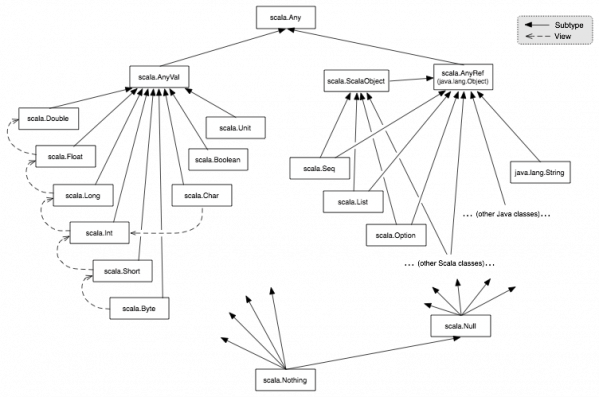
\includegraphics[width=10cm]{scala_type_hierarchy}
\caption{scala type hierarchy}
\end{figure}


\begin{itemize}
\item { \bf Any} is the base type of all types.
\item {\bf AnyVal} inherits from Any. Numeric types (boolean, Int) inherit from AnyVal
\item {\bf Any} defines methods '==','!=', toString
\end{itemize}

Nothing is at the bottom of scala's type hierarchy. it is a subtype of every other type.
Nothing can signal abnormal termination.
Empty lists/containers can have elememt type Nothing

Null is a subtype of all reference types, and the type of the null value
(null is the value, Null is the type)

% term rewriting?

% Class hierarchies - more than one class goes into the definintion of a derived class





% syntax notation
% extended Backus-Naur form (EBNF)






\part{Program Design}
\chapter{more with for}
\section{queries with for}

For expresions in scala can be likened to queries in an RDBMS.

\begin{lstlisting}
for (b <-books, a<- b.authors if a.startsWith "Bird," ) yield b.title

for { 
	b1 <- books
	b2 <- books
	if b1.title < b2.title
	a1 <- b1.authors
	a2 <- b2.authors
	if a1 == a2
	} yield a1
\end{lstlisting}

If the author has written 3 books, they will be printed 3 times.

\section{translating for-expressions}
For expressions are pretty handy. For expressions can generally be translated into expressions based on flatmap, map, and filter. Conversely, all of these functions can be defined in terms of for - 
\begin{lstlisting}
def mapFun[T,U](xs: List[T], f: T => U) : List[U] = for (x <- xs) yield f(x)

def flatMapFun[T,U]( xs:List[T], f: T => List[U]): List[U] = for (x <- xs, y <- f(x)) yield y

def filterFun[T](xs: List[T], f: T => Boolean): List[T] = for (x <-xs if f(x)) yield x

\end{lstlisting}

Scala translates for expressions into expressions based on map, flatmap and filter.

A really simple for-expression
\begin{lstlisting}
for (x <-e1) yield e2
\end{lstlisting}
can be translated to
\begin{lstlisting}
e1.map( x => e2)
\end{lstlisting}

Expressions of the form \lstinline|for (x <-e1 if f; s) yield e2|, where f is a filter and s is a (potentially empty) arbitrary sequence of generators and filters can be translated to 
\begin{lstlisting}
for (x<- e1.withFilter(x => f) ; s ) yield e2
\end{lstlisting}
withfilter is a lazy (i.e. smarter) implementation of filter. It does not create a new (intermediate) collection. The above expression is still contains a for expression, but we have removed one element (the if).

Cases containing more than one leading generator can be translated using flatmap
\begin{lstlisting}
for (x <-e1 ; y<-e2 ; s) yield e3
\end{lstlisting}
can be translated to 
\begin{lstlisting}
e1.flatMap(x => for (y <-e2 ; s) yield e3
\end{lstlisting}

In all of these cases, we are removing one element from the for expression. Thus an arbitrary expression can be reduced to a sequence of maps and flatmaps.

\begin{lstlisting}
for { 
	i <- 1 to N
	j <- 1 to i
	if isPrime(i + j)
} yield (i, j)
\end{lstlisting}

can be rewritten as
\begin{lstlisting}
//(1 until N).flatMap(i => for ( y <- 1 until i if isPrime(i,j)) yield (i,j) )

(1 until N).flatMap( i => 
	(1 until i).withFilter(j => isPrime(i + j)
	.map(j => (i,j)))
\end{lstlisting}

The for query above on books can be translated to \lstinline|books.flatmap(b => b.authors.withFilter(a => a.startswith("Bird").map(y => y.title)))|

Note that for expressions are not limited to lists//sequences/iterables. The translation only depends on the prescence of the methods map, flatmap, and withFilter. User defined types can be used in for expressions, provided these three methods are implemented.

For example, the collection books might instead be an interface to a database. Provided the methods are are implemented, for expressions can be used to query. the Scala database connection frameworks ScalaQuery and Slick make use of this.



\section{Monads}

monads must have an associated unit function, and have a flatmap method. I don't really get monads right now.

\section{Structural Induction}

Structural induction can be applied to trees.
To prove a property $P(t)$ for all trees of a certain type $t$
\begin{itemize}
	\item show that $P(l)$ holds for all leaves $l$ of a tree
	\item For each type of internal node t with subtrees $s_1, s_2 \ldots s_n$, show that
	$P(s_1)\wedge P(s_2)\wedge \ldots \wedge P(s_n)$ implies $P(t)$ 
\end{itemize}

if the property holds on all of the tree's subtrees, then it holds on the tree


consider the implementation of IntSets

\begin{lstlisting}
abstract class IntSet {
	def incl(x: Int) : IntSet
	def contains(x: Int): Boolean
}

object Empty extends IntSet {
	def contains(x: Int): Boolean = false
	def incl(x: Int): IntSet = NonEmpty(x, Empty, Empty)
}

case class NonEmpty(elem: Int, left: IntSet, right: IntSet) extends IntSet {
	def contains(x: Int): Boolean = 
		if (x < elem) left contains x
		else if (x > elem) right contains x
		else true
	def incl(x: Int): IntSet = 
		if  (x < elem) NonEmpty(elem, left incl x, right)
		else if (x > elem) NonEmpty(elem, left, right incl x)
		else this
}
\end{lstlisting}

how do we prove the correctness of this implementation holds? 
consider the following three laws (for integers x,y and Intset s):
\begin{itemize}
	\item \lstinline|Empty contains x = false|
	\item \lstinline| (s incl x) contains x = true|
	\item \lstinline|(s incl x) contains y = s contains y|
\end{itemize}

The first law is straightforward, and can be seen to be true (Empty.contains is false). 

For the second law (proposition), we can do strutural induction. Consider the base case when $s$ is an empty set. The we would like to show that \lstinline| (Empty incl x) contains x = true|. \lstinline|Empty incl x| evaluates to \lstinline| NonEmpty(x,...)|, and contains x will evaluate to true in this case.

For the base case when $s$ is NonEmpty, assume it takes the form NonEmpty(z,l,r), where l and r are subtrees. There are two cases to consider, z == x and z != x. If z == x, then NonEmpty(x,...) incl x will return this, which contains x, so we're good. if z != x, then NonEmpty(z) incl x will contain x, so we're good.
\section{streams}

Streams are like lists, but are evaluated lazily. The tail of the stream is not evaluated until it is needed. Streams are constructed from the object Stream.empty and the constructor stream.cons.

For lists, we might have something like
\begin{lstlisting}
def listrange(lo:Int, hi: Int): List[Int] = 
	if lo >= hi Nil
	else lo::listrange(lo+1,hi)
\end{lstlisting}
For streams, we would do
\begin{lstlisting}
def StreamRange(lo:Int, hi: Int): Stream[Int] = 
	if lo >= hi Stream.empty
	else Stream.cons(lo,StreamRange(lo+1,hi))
\end{lstlisting}

The standard shorthand for the cons operator, \lstinline|::|, will always produce a list. There is an equivalent for streams, the hash operator: \lstinline|#::|, which can be used in expressions and patterns. 

\section{State}
Up untill now we've been doing this purely functionally, as much as possible.
Some things will have a state. 

Everything witha mutable state will be constructed from variables. variables are declared with \lstinline|var| instead of \lstinline|val|. Variables can have their value changed later through assignment.

When assignment is possible, then determining whether or not things are equivalent becomes more difficult. Previously, if things evaluate to the same expression, then they are equal. 

\begin{lstlisting}
val x = E; val y = E;
val x = E; val y = x;
\end{lstlisting}
The two lines above produce the same result. In both cases, x and y evaluate to E
\begin{lstlisting}
val x = new BankAccount; val y = new BankAccount;
val x = new BankAccount; val y = x;
\end{lstlisting}
In this case, the two lines give different results. In the first, two new bankaccounts are created. In the second, y is copied from x.

How do we define "the same"? Operational equivalence - Execute the definitions of x and y, followed by an arbitrary set of operations involving x and y (S), observing all results. Then, execute the definitions followed by a different sequence of operations, S', in which every occurence of y in S has been replaced by x. If the results are different, then x and y are certainly different. Else, if every possible pair of sequences (S, S') are indistinguishable, then x and y are the same.

Assignment breaks the substitution model that we have been using up until now. In general, if we are not using purely functional code, then the substitution model will not hold.

\section{Loops}

Here's a possible definition of while that can be used to constrruct loops
\begin{lstlisting}

def WHILE(condition: => Boolean)(command :=> unit): unit = 
	if condition
	{ command
		WHILE(condition)(command)
		}
	else ()
\end{lstlisting}

 \section{event simulation}

 digital circuits - states are boolean.
 Will consider inverters (NOT), AND, and OR gates.

 Half adder - takes two inputs (A and B), and has two outputs (SUM and CARRY). CARRY is equal to A AND B, while SUM is A OR B AND NOT A AND B


\begin{figure}
\begin{circuitikz}
\draw 

(2,0) node[and port] (lowerand) {} 
(2,3) node[or port] (upperor) {}

(upperor.in 1) -- ++ (-2,0)
(lowerand.in 2) -- ++ (-2,0)

(upperor.out) ++( 2,0) node[and port, anchor=in 1](upperand){}
(lowerand.out) |- ++(1,1) node[not port](middlenot){}
(middlenot.out) |- (upperand.in 2)
(upperor.out) -- (upperand.in 1)

(upperor.in 1) -- ++ (-1.25,0) |- (lowerand.in 1)
(upperor.in 2) -- ++ (-0.75,0) |- (lowerand.in 2)
(lowerand.out) -- ++ (4,0)
;

\end{circuitikz}
\caption{half adder}
\end{figure}

two half adders can be combined (with an or gate) to form a full one-bit adder

\begin{figure}
\begin{circuitikz}
\draw 

(1,0) node[fourport, label=HA1] (ha1) {} 

(ha1.4) ++ (3,0) node[fourport,t=HA2, anchor=1] (ha2) {}
(ha2.2) ++ (1,0) node[or port,t=or, anchor=in 1] (or1) {}

(ha1.1) ++ (-1,0) node[ocirc](cin){Cin}
(ha1.4) ++ (-1,0) node[ocirc](a){A}
(ha2.4) ++ (-4,0) node[ocirc](b){B}
(ha2.3) ++ (3,0) node[ocirc](sum){Sum}
(or1.out) ++ (1,0) node[ocirc](carry){Cout}


(ha1.3) -- (ha2.1)
(ha2.2) -- (or1.in 1)
(ha1.2) -| (or1.in 2)

(cin) -- (ha1.1)
(a) -- (ha1.4)
(b) -- (ha2.4)
(ha2.3) -- (sum)
(or1.out) -- (carry)

;

\end{circuitikz}
\caption{full 1-bit adder}
\end{figure}

\subsection{event handling}

Oberver pattern, also called publish/subscribe or model/view/controller. Views { \em subscribe} to the model. When the something in the model changes, it { \em publishes} an update, sending the update to all subscribed views. 

\begin{lstlisting}
trait Publisher {
	private var subscribers: Set[Subscriber] = Set()

	def subscribe(subscriber:Subscriber): Unit = 
		subscribers += subscriber

	def unsubscribe(subscriber:Subscriber): Unit = 
		subscribers -= subscriber

	def publish(): Unit = 
		subscribers.foreach(_.handler(this))
}
\end{lstlisting}

Our BanAccount class could extend from Publisher, and then it would be able to inform other parts of the application when changes to the balance occur

\begin{lstlisting}
class BankAccount extends Publisher {
	private var balance = 0
	def currentBalance:Int = balance

	def deposit(amount:Int):Unit = 
		if (amount > 0) 
		{
			balance = balance + amount
			publish()
		}

	def withdraw(amount:Int):Unit = 
		if (amount > 0 && balance >= amount) {
		balance = balance - amount
		publish()
		} else throw new Error("insufficient funds")
}
\end{lstlisting }

The balance can be queried through currentBalance, and any changes (deposits/withdrawals) are published to observers
Speaking of observers

\begin{lstlisting}

class Consolidator(observed: List[BankAccount]) extends Subscriber {
	observed.foreach(_.subscribe(this))

	private var total: Int = _
	compute()

	private def compute() =
		total =  observed.map(_.currentBalance).sum

	def handler(pub: Publisher) = compute()

	def totalBalance = total

}
\end{lstlisting}

The observer pattern (good points)
\begin{itemize}
	\item is simple to set up
	\item decouples views from state
	\item allows multiple views of the same (or similar) states
\end{itemize}

but (bad points)
\begin{itemize}
	\item forces imperative style (handlers are unit functions)
	\item lots of moving parts that need to be coupled
	\item concurrency makes things complicated
\end{itemize}

\subsection{functional reactive programming}
reactive programming is reacting to a sequence of events in time.

Functionally, we aggregate an event sequence into a signal.
\begin{itemize}
	\item The signal is a value that changes over time.
	\item it is represented as a function that maps from time domain to value.
	\item instead of propagating updates to a mutable state, we define new signals in terms of existing ones.
\end{itemize}

There are two fundamental operations over signals - obtaining the value of the signal at the current time, e.g. \lstinline|mousePosition()| and defining a signal in terms of other signals -
\begin{lstlisting}

def inReactangle(LL: Position, UR: Position): Signal[Boolean] = 
Signal {
	val pos = mousePosition()
	LL <= pos && pos <= UR
}
\end{lstlisting}

Values of Signal are immutable
There is a subclass of Signal, \lstinline|Var|, that has an update operation
\begin{lstlisting}
val sig = Var(3) // signal with constant value of 3
sig.update(5) // sig now has value of 5
\end{lstlisting}

Updates can be written as assignments (syntactic sugar).
Variable signals look a bit like mutable variable, but we can map over them. If we define a signal b to be equal to 2 time a, then updates to a automatically propagate to b. With mutable variables this is not the case, b would need to be redefined after a is changed.

bank account with signals looks much simpler. no need to explicitly publish stuff.
\begin{lstlisting}
class BankAccount {
	val balance = Var(0)
	
	def deposit(amount:Int):Unit = 
		if (amount > 0) 
		{
			balance() = balance() + amount
			// syntatic sugar for balance.update(balance() + amount)
		}

	def withdraw(amount:Int):Unit = 
		if (amount > 0 && balance() >= amount) {
		balance() = balance() - amount
		} else throw new Error("insufficient funds")
}
\end{lstlisting }


\section{more functional reactive programming}

\url{https://github.com/rohgar/scala-design-2/wiki/A-Simple-FRP-Implementation}

signals take an expression, and implement an apply method
\begin{lstlisting}
class Signal[T]( expr: => T) {
    def apply(): T = ??? 
}

object Signal {
    def apply[T] (expr: => T) = new Signal(expr)
}
\end{lstlisting}
\lstinline|Signal(expr)|will invoke the object's apply method, returning a new instance of the Signal class, with the supplied expression.

Vars extend signals, such that they can be updated. Vars implement and update method.

\begin{lstlisting}
class Var[T] (expr: => T) extends Signal[T](expr) {
    def update(expr: => T): Unit = ???
}

object Var { 
    def apply[T](expr: => T) = new Var(expr)
}

moose = Var(expr)
moose.update(expr2)
\end{lstlisting}

\subsection{Syntatic sugar}
\lstinline|moose() = expr2| is equivalent to \lstinline|moose.update(expr2)|, just as \lstinline|moose(expr)| is syntatic sugar for \lstinline|moose.apply(expr)|.


signal maintains:
\begin{itemize}
\item it\'s current value
\item the expression that defines the signal value
\item a set of observers - other signals that depend on value.
\end{itemize}
if signal changes, observers are re-evaluated.


How do we record dependencies?

\section{latency/asynchoronicity}
Computations can take time. 
Scala has a Try monad for exception handling. Try is an abstract class with Success and Failure case subclasses. We can iterate over stuff, and return an instance of success when it works or Failure when it does not. Then we can make use of the successes and handle the failures.

Future is another monad, Instead of handling success/failure it handles latency - the computation may be complete or ongoing (or waiting/whatever)

Really simple network stack:
\begin{lstlisting}
trait Socket {
	def readFromMemory(): Array[Byte]
	def sendToEuropet(packet: Array[Byte]): Array[Byte]
	}

val socket = Socket()
val packet = socket.readFromMemory()
val confirmation = socket.sendToEurope(packet)

\end{lstlisting}
Reading from memory takes some time, sending to Europe takes a lot of time.

\lstinline{Future[T]} is a monda that handles both Exceptions and Latency.

\begin{lstlisting}

import scala.concurrent._
import scala.concurrent.Execution.Implicits.global

trait Future[T] {
	def onComplete(callback: Try[T] => Unit)
	//(implicit executor: ExecutionContext): Unit
}
\end{lstlisting}

When the execution is complete, the callback function is invoked. Note that as the try monad is used, the computiation we are waiting for may have suceeded or failed, but this can be handled.

Javascript uses a shit-tonne of callbacks.

Our reading/sending example above can be modified to 
\begin{lstlisting}

val socket = Socket()
val packet: Future[Array[Byte]] = socket.readFromMemory()

val confirmation: Future[Array[Byte]] = packet.onComplete{
	case Sucess(p) => socket.sendToEurope(p)
	case Failure(t) => ...
	}
\end{lstlisting}

This can result in a lot of nesting. But monads are sweet, because they can be flatmapped.

The implementation of Future might look like
\begin{lstlisting}
trait Future[T] {
	def onComplete( callback: Try[T] => unit) = ...
	def flatMap[S] (f: T => Future[S]) : Future[S] = ???
}
\end{lstlisting}
How would we implement flatMap using onComplete? 

\begin{lstlisting}
trait Future[T] { self => 
	def flatMap( f: T => Future[S]): Future[S] = { 
		new Future[S]{
			def onComplete(callback: Try[S] => Unit): Unit = {
				self onComplete {
					case Success(x) => f(x).onComplete(callback)
					case Failure(e) => callback(Failure(e))
				}
			}
		}
	}
}
\end{lstlisting}

Flatmap creates a new \lstinline|Future[S]|, and defines it's onComplete method. The new future's oncomplete relies on the onComplete method of the initial Future (self). If the self computation completes sucessfully, then the mapping function f is applied and the onComplete/callback for the Future[S] is invoked.
if self's computation fails, then the failure is passed to the callback function directly.




\part{parallel programming}
\chapter{parallel programming}

parallelism and concurrency

parallelism is doing several things at the same time, by efficently using hardware
parallelism is mainly concerned with organising the computational prbolem into multiple subproblems that can be executed simultaneously and independently.
parallel programming focusses on structuring the algorithms and/or data, such that as many numbers can be crunched as quickly as possible.

Bit-level parallelism is structuring the hardware/software so that a larger number of bits are involved in a single operation. Think of addition - one bit addition would add the ones bits, then carry over (if needed) and add the twos bits, then carry over and do the fours bits, and so on. Alternatively, a four bit algorithm/hardware could add all four of these bits simultaneously in a single operation.

Instruction level parallelism is executing different instructions from the same instruction stream in parallel

concurrency is where multiple instructions may or may not execute at the same time.
Main focus of conncurrency is figuring out how to structure a program such that some parts can continue to execute while other parts wait for things (fetch data from memory/disk/database/web). Concurrent programming is targeted towards writing asynchrounous applications.

There is some overlap between the two, but neither is a superset of the other.


c = a2 + a2
b = a1 + a2
d = b + c

b and c can be computed in parallel. This is instruction level parallelism

task level parallism - carrying out operations from two (or more) seperate instruction streams at the same time.
THis is what we deal with mostly.

\section{paralleism in the jvm}

will assume we are running on a multicore/multiprocessor system

\begin{itemize}
    \item OS - software that manages hardware and software resources, and schedules program execution
    \item process - an instance of a program
    \begin{itemize}
        \item The same program can be started more than once, and thus may be running in multiple processes
    \end{itemize}
    \item threads

\end{itemize}

There are usually many processes running on a small number of cpus. The OS schedules execution - each process will run for a small chunk of time ( {\em time slice}), then the os switches execution to another. This is multitasking.

two different processes cannot directly access each other's memory - they are isolated.

A single program (process) may make use of multiple threads (concurrency units). All threads within a program have access to the program's memory space.

Each thread has a program counter and a program stack. A given thread may not access the stack (or stack variables) of another thread. For threads to communicate, they must read/write to shared (heap) memory.

\section{threading in the jvm}

\begin{itemize}
    \item define a subclass of \lstinline|Thread|
    \item instantiate an object of this subclass
    \item invoke the \lstinline|start| method of the subclass
\end{itemize}

The definition of the subclass defines the code that will be used. 

An operation is {\em atomic} if it occurs instantaenously from the perspective of other threads.
The \lstinline|synchronized| block can be invoked to ensure atomicity. No more than one thread may execute the same synchronized block at the same time.

synchronized blocks can be nested. For example, when transferring from a source to a destination, you might want to invoke synchoronised on both objects, such that the transfer is atomic.

\section{deadlock}
Deadlock occurs when two (or more) threads wait to acquire resources without releasing resources that they hold. None of the threads can proceed, as all are waiting for another thread to finish. This can happen when \lstinline|synchronized| blocks are nested.

Deadlocks can be avoided by always acquiring resources in a specific order. In the transfer example, each account is associated with a unique id. For a given transfer, the lowest uid is acquired first, followed by the other. This avoids circular dependencies, as things hold the lowest and wait for the highest. Assuming self-transfers are guarded against, then one of the threads involving the highest account will be able to complete, freeing the lower, allowing other threads to proceed. 

\section{memory model}
the memory model is a set of rules used in the JVM that describes how threads will interact when accessing shared memory.

\begin{itemize}
    \item two threads writing to seperate locations do not require synchronisation
    \item A thread X that joins on thread Y is guaranteed to observe all writes performed by Y after join returns.
\end{itemize}

Threads and Synchronization are fairly low level functionalities. In practice we will probably work with higher level abstractions.


\section{running computations in parallel}

Consider the case where we want to compute the pnorm for an array

\begin{equation}
\norm{\mathbf{x}}_p = \left(\sum_{i=1}^{n} |x_i|^p \right)^{1/p}
\end{equation}


Simplest case is to just sequentially loop over all the elements.
We can use two threads. Define $m=n/2$, then one thread computes the sum for $1 \leq i < m$, the other for $m \leq i \leq n$. Then we add the results and raise to the power $1/p$.

Following will compute the sum of the raised elements of an array (worksheet pnorm)
{\bf Note} - the ending index on slice is exclusive.
\begin{lstlisting}
def sumSegment(a: Array[Int], p:Double, s: Int, t:Int): Int =
  {
    def raise(aa:Int): Int = floor(pow(aa.abs,p)).toInt

    a.slice(s,t).map(raise).sum
  }

val myArray = Array(1,2,3,4,5,6)

sumSegment(myArray,2,0,3)
\end{lstlisting}

Four four threads, we could similarly divide the initial array into four pieces. What if we have an unbounded number of threads? If there is no predefined limit on the number of threads we may use, then we can break this into as many pieces as is suitable. There is some overhead associated with setting up threads, so we define some threshold. For a (sub) array with size less than the threshold, we just operate on it sequentially, else we break our array into two pieces and parallelise across these.

\begin{lstlisting}

def pNormRec(a: Array[Int],p:Double): Int = 
    power(segmentRec(a,p,0,a.length),1/p)

def segmentRec(a: Array[Int],p: Double,s: Int,t: Int) = {
    if (t-s < threshold)
        sumSegment(a,p,s,t)
    else
    {
    val m = s + (t - s)/2 // (t +s) /2 ?
    val sum1, sum2 = parallel(
        segmentRec(a,p,s,m),
        segmentRec(a,p,m,t))
    sum1 +sum2
    }

}
\end{lstlisting}
Again, note that as the ending index on slice is exclusive, we can specify $m$ as both the end index for the first segment and the start index for the second segment.

\section{first class tasks}
Previously considered a construct, parallel, that would evaluate expressions in parallel
\begin{lstlisting}
val (v1,v2) = parallel(e1,e2)
\end{lstlisting}

Alternatively, we could use a task construct.
\begin{lstlisting}

val t1 = task(e1) // spawns a new thread computing e1
val t2 = task(e2) // spawns a new thread computing e2
val v1 = t1.join // joins t1, obtaining result v1 (waits till t1 thread completes)
val v2 = t2.join // joins t2 with result v2

\end{lstlisting}

When creating the tasks, the current computation (presumably the main thread) continues. The join calls are { \em blocking} - the main thread above will wait until task t1 concludes. Subsequent calls to t1.join quickly return the same result.


parallel can be expressed in terms of task
\begin{lstlisting}
def parallel[A,B](cA: => A, cB: => B): (A,B) = {
    //val ta = task cA
    val tb = task cB
    //(ta.join, tb.join)
    val aa = cA
    (aa,tb.join)

    }

\end{lstlisting}


Note that the "task" construct that is mentioned here is implemented in the assignment. The task and parallel implemtations wrap functionality from \lstinline|java.util.concurrent| (ForkJoinTask).

\section{complexity of parallel programs}
W(e) - the work of a sequential program (single thread)
treat parallel as pair - parallel(e1,e2) -> (e1,e2)
D(e) - the depth of a parallel program (or span) - the number of steps it would be broken into given unbounded parallelism.

W(parallel(e1,e2)) = W(e1) + W(e2) + c1
D(parallel(e1,e2)) = max(D(e1),D(e2)) + c2

If work is divided into equal parts, for depth we only count one part.
for parts where we do not explicitly call parallel, we add the constituents

Suppose our platform has P processors. The fastest we could do all the work is W(e)/P
Suppose we had unbounded parallelism (infinite threads). The fastest we could do everything is D(e)

D(e) + W(e)/P is often used as an estimate for running time. Given W and D, we can estimate how performance time will behave for different P. If P is constant but inputs grow, then the running time scales linearly with the size of the inputs.
Even with infinite resources, we are still bounded by D(e).

\subsection{Amahl's law}

Suppose a program has two parts. part $p_1$ takes 40\% of the time, while part $p_2$ takes the reamining 60\% of the time, but can be sped up. If we make part 2 faster by $P$ times, the speedup for the entire program is

\begin{equation}
S = \frac{1}{f + \frac{1-f}{p}}
\end{equation}

which tends to $1/f$ as $P \rightarrow \infty$.


\section{parallel sorting}

\subsection{Merge sort}
This is interesting, as it's not a pure merge sort. Paralleisation is a function of the depth at which we're operating - if we are up high, then we split the array and create new threads. Once a sufficient depth has been reached, we stop spawning new threads. However, instead of doing a mergesort sequentially, we change the algorithm to a quickSort, which operates sequentially.

Sorting is done in place, but auxillary storage is used for merging. At each depth level, we alternate between merging from xs into ys with merging from ys into xs.

\begin{lstlisting}

def parMergeSort(xs: Array[Int, maxDepth:Int): Unit = {
    // aux storage
    val ys = new Array[Int](xs.length)

    def sort(from: Int, until: Int, depth:Int) = {
        if (depth == maxDepth) {
            quickSort(xs, from, until - from)
        } else {
            val mid = (from + until)/2
            parallel(sort(from,mid,depth+1),sort(mid,until,depth+1))

            val flip = depth %2 == 0
            val src = if (flip) ys else xs
            val dst = if (flip) xs else ys
            merge(src,dst,from,mid,until)
        }
    }
}
\end{lstlisting}

\subsection{parrallel operations on collections}

operations on collections (such as map, fold, scan) are pretty foundational to functional programming.

scan 
List(1,3,8).scan(100)((s,x) => s + x ) == List(100, 101, 104, 112)

like zip + fold? can think of scan as applying fold to all list prefixes, or storing the intermediate results of fold

List is not an ideal data structure for parallel computations, as we need to search through the list to find the middle. concatenation also takes linear time.

\subsection{Fold Operations}

Map applies an operation to each element in the sequence. Fold uses a reduction operator (and an initial value) to combine elements, returning a single result. FoldLeft and FoldRight start at the beginning and end of the sequence, respectively. 

The result of a fold operation can depend on the order in which the operation is applied to the collection. 
\begin{lstlisting}
List(1,3,8).foldLeft(100)((s,x) => s - x) == (((100 -1) -3) -8) == 88
List(1,3,8).foldRight(100)((s,x) => s - x) == (1- (3 - (8 - 100))) == -94
\end{lstlisting}

To enable parallel operations on collections, we consider associative operations - the order of the operations does not matter
\begin{eqnarray*}
f(a,f(b,c)) & = & f(f(a,b),c) \\
1 + (2 + 3) & = & (1 + 2) + 3 \\
1 - (2 -3) & \nequal & (1 -2) -3 \\
\end{eqnarray*}
Addition (and multiplication) are associative, whereas subtraction and division are not. Multiplication is commutative also, in that $ f(a,b) = f(b,a)$, whereas division and subtraction are not. String concatenation is also associative.

The operation $f(a,b)$ can be written in infix form $ a \circlex b$. A sequence of these operations can be written in the form of a tree, where the leaves are values and nodes are $\circledot$. 


% \begin{lstlisting}
% // Hello.java
% import javax.swing.JApplet;
% import java.awt.Graphics;

% public class Hello extends JApplet {
%     public void paintComponent(Graphics g) {
%         g.drawString("Hello, world!", 65, 95);
%     }    
% }
% \end{lstlisting}


\end{document}
